%
% chapter.tex
%
% (c) 2020 Prof Dr Andreas Müller
%
\chapter{Integration\label{chapter:integration}}
\lhead{Integration}
\rhead{}
\index{Integration}%
Die Wahrscheinlichkeitsdichte der Standardnormalverteilung führt 
auf das Integral
\index{Integral}%
\[
\Phi(x) 
=
\frac{1}{\sqrt{2\pi}}
\int_{-\infty}^x e^{-t^2/2}\,dt
\]
für die Verteilungsfunktion.
\index{Verteilungsfunktion}%
\index{Normalverteilung}%
\index{Standardnormalverteilung}%
Man kann beweisen, dass es für diesen Integranden keine Stammfunktion
in analytischer Form als algebraischer Ausdruck bekannter Funktionen
geben kann.
Es bleibt also nur die numerische Berechnung.
Dieses Kapitel stellt einige Methoden zur Berechnung von Integralen
zusammen. 

%
% riemann.tex -- Definition des Integrals mit Hilfe der Riemann-Summe
%
% (c) 2020 Prof Dr Andreas Müller, Hochschule Rapperswil
%
\documentclass[tikz]{standalone}
\usepackage{amsmath}
\usepackage{times}
\usepackage{txfonts}
\usepackage{pgfplots}
\usepackage{csvsimple}
\usetikzlibrary{arrows,intersections,math}
\begin{document}
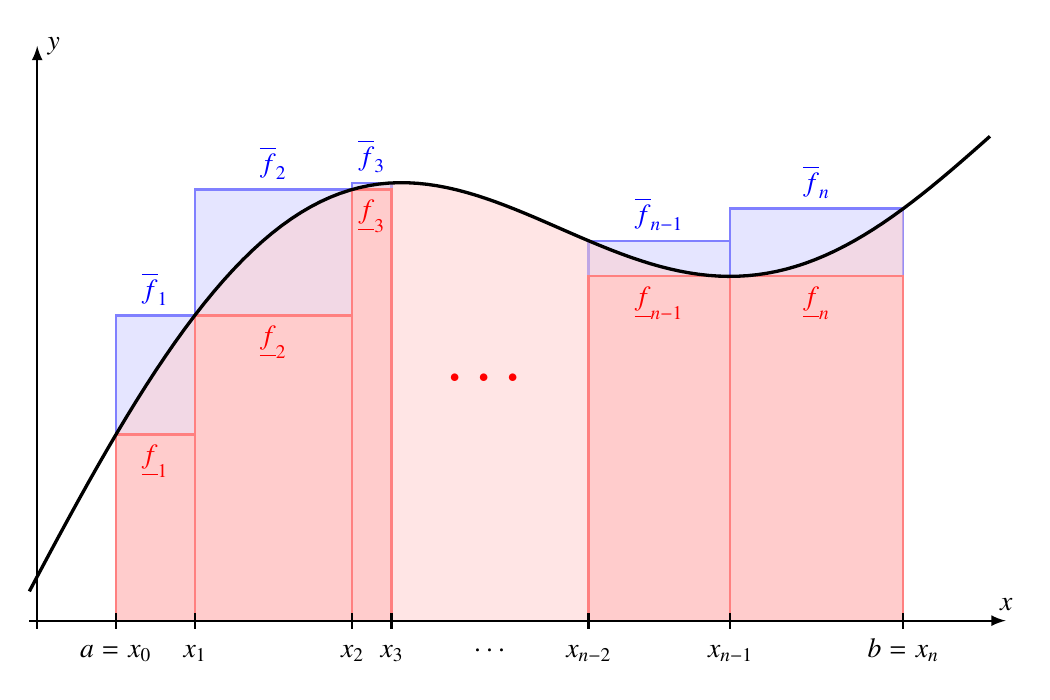
\begin{tikzpicture}[>=latex,thick]

\def\A{2}
\def\B{0.5}
\def\C{0.04}
\def\D{1.8}

\def\a{1}
\def\xone{2}
\def\xtwo{4}
\def\xthree{4.5}
\def\xminustwo{7}
\def\xminus{8.8}
\def\b{11}

\def\oberesrechteck#1#2#3#4{
	\fill[color=blue!10] (#1,0)--(#2,0)--(#2,#3)--(#1,#3)--cycle;
	\draw[color=blue!50] (#1,0)--(#2,0)--(#2,#3)--(#1,#3)--cycle;
	\node[color=blue] at ({0.5*(#1+#2)},{#3}) [above] {#4};
}

\def\unteresrechteck#1#2#3#4{
	\fill[color=red!20] (#1,0)--(#2,0)--(#2,#3)--(#1,#3)--cycle;
	\draw[color=red!50] (#1,0)--(#2,0)--(#2,#3)--(#1,#3)--cycle;
	\node[color=red] at ({0.5*(#1+#2)},{#3}) [below] {#4};
}

\oberesrechteck{\a}{\xone}{{\A+\B*\xone-\C*(\xone-6)*(\xone-6)+\D*sin(90*\xone/3.14)}}{$\overline{f}_1$};
\oberesrechteck{\xone}{\xtwo}{{\A+\B*\xtwo-\C*(\xtwo-6)*(\xtwo-6)+\D*sin(90*\xtwo/3.14)}}{$\overline{f}_2$};
\oberesrechteck{\xtwo}{\xthree}{{\A+\B*\xthree-\C*(\xthree-6)*(\xthree-6)+\D*sin(90*\xthree/3.14)}}{$\overline{f}_3$};

\oberesrechteck{\xminustwo}{\xminus}{{\A+\B*\xminustwo-\C*(\xminustwo-6)*(\xminustwo-6)+\D*sin(90*\xminustwo/3.14)}}{$\overline{f}_{n-1}$};
\oberesrechteck{\xminus}{\b}{{\A+\B*\b-\C*(\b-6)*(\b-6)+\D*sin(90*\b/3.14)}}{$\overline{f}_n$};

\fill[color=red!20,opacity=0.5]
	plot[domain=1:11,samples=100]
		(\x,{\A+\B*\x-\C*(\x-6)*(\x-6)+\D*sin(90*\x/3.14)})
	-- (\b,0)--(\a,0)--cycle;

\unteresrechteck{\a}{\xone}{{\A+\B*\a-\C*(\a-6)*(\a-6)+\D*sin(90*\a/3.14)}}{$\underline{f}_1$}
\unteresrechteck{\xone}{\xtwo}{{\A+\B*\xone-\C*(\xone-6)*(\xone-6)+\D*sin(90*\xone/3.14)}}{$\underline{f}_2$}
\unteresrechteck{\xtwo}{\xthree}{{\A+\B*\xtwo-\C*(\xtwo-6)*(\xtwo-6)+\D*sin(90*\xtwo/3.14)}}{$\underline{f}_3$}

\unteresrechteck{\xminustwo}{\xminus}{{\A+\B*\xminus-\C*(\xminus-6)*(\xminus-6)+\D*sin(90*\xminus/3.14)}}{$\underline{f}_{n-1}$}
\unteresrechteck{\xminus}{\b}{{\A+\B*\xminus-\C*(\xminus-6)*(\xminus-6)+\D*sin(90*\xminus/3.14)}}{$\underline{f}_n$}

\draw[line width=1.2pt] plot[domain=-0.1:12.1,samples=100]
	(\x,{\A+\B*\x-\C*(\x-6)*(\x-6)+\D*sin(90*\x/3.14)});


% add image content here
\draw[->] (-0.1,0)--(12.3,0) coordinate[label={$x$}];
\draw[->] (0,-0.1)--(0,7.3) coordinate[label={right:$y$}];

\draw (\a,-0.1)--(\a,0.1); \node at (\a,-0.1) [below] {$\mathstrut a=x_0$};
\draw (\b,-0.1)--(\b,0.1); \node at (\b,-0.1) [below] {$\mathstrut b=x_n$};

\draw (\xone,-0.1)--(\xone,0.1);
\node at (\xone,-0.1) [below] {$\mathstrut x_1$};

\draw (\xtwo,-0.1)--(\xtwo,0.1);
\node at (\xtwo,-0.1) [below] {$\mathstrut x_2$};

\draw (\xthree,-0.1)--(\xthree,0.1);
\node at (\xthree,-0.1) [below] {$\mathstrut x_3$};

\node at (5.75,-0.1) [below] {$\mathstrut\cdots$};
\node[color=red] at (5.75,3) {\Huge$\cdots$};

\draw (\xminustwo,-0.1)--(\xminustwo,0.1);
\node at (\xminustwo,-0.1) [below] {$\mathstrut x_{n-2}$};

\draw (\xminus,-0.1)--(\xminus,0.1);
\node at (\xminus,-0.1) [below] {$\mathstrut x_{n-1}$};

\end{tikzpicture}
\end{document}


%
% romberg.tex
%
% (c) 2020 Prof Dr Andreas Müller, Hochschule Rapperswil
%
\begin{frame}
\frametitle{Konvergenz-Beschleunigung}
\vspace{-15pt}
\begin{columns}[t]
\begin{column}{0.42\hsize}
\begin{block}{Idee}
Fehlergesetz $\Rightarrow$ Fehler wegrechnen
\end{block}
\uncover<2->{%
\begin{block}{Fehler}
\vspace{-15pt}
\begin{align*}
I&=T(h) + Ch^2&&\uncover<3->{|\;\cdot (-1)}
\\
I&=T({\textstyle\frac{h}2}) + C\frac{h^2}4 &&\uncover<3->{|\;\cdot 4}
\\
\uncover<4->{3I}&\uncover<4->{=4T({\textstyle\frac{h}2}) - T(h)}
\end{align*}
\end{block}}
\vspace{-10pt}
\uncover<5->{%
\begin{block}{Konvergenzverbesserung}
\[
T^*({\textstyle\frac{h}2})
=
\frac{4T({\textstyle\frac{h}2})-T(h)}3
\]
\end{block}}
\end{column}
\begin{column}{0.54\hsize}
\uncover<6->{%
\begin{block}{Allgemein}
\vspace{-15pt}
\begin{align*}
T^{*0}(h) &= T(h)
\\
T^{*k}(h) &= \frac{4^kT^{*(k-1)}({\textstyle\frac{h}2}) - T^{*(k-1)}(h)}{4^k-1}
\end{align*}
\end{block}}
\vspace{-10pt}
\uncover<7->{%
\begin{block}{Romberg-Schema}
%\vspace{-10pt}
\begin{center}
\begin{tabular}{>{$}c<{$}|>{$}c<{$}>{$}c<{$}>{$}c<{$}}
T(2^{\phantom{-}0})&               &                            &               \\
T(2^{-1})&\uncover<8->{T^*(2^{-1})}&                            &               \\
T(2^{-2})&\uncover<8->{T^*(2^{-2})}&\uncover<9->{T^{**}(2^{-2})}&               \\
T(2^{-3})&\uncover<8->{T^*(2^{-3})}&\uncover<9->{T^{**}(2^{-3})}&\uncover<10->{T^{***}(2^{-3})}\\[8pt]
O(h^2)   &\uncover<8->{O(h^4)     }&\uncover<9->{O(h^6)        }&\uncover<10->{O(h^8)}
\end{tabular}
\end{center}
\end{block}}
\end{column}
\end{columns}
\end{frame}

%
% andere.tex
%
% (c) 2020 Prof Dr Andreas Müller, Hochschule Rapperswil
%
\section{Weitere Integrationsverfahren
\label{buch:section:weitereintegrationsverfahren}}
\rhead{Weitere Integrationsverfahren}
Die bisher vorgestellten Verfahren haben vor allem den Mangel, dass
die Zahl der Funktionsauswertungen sehr gross wird, wenn eine
hohe Genauigkeit angestrebt wird.
Das Verfahren der {\em Gauss-Quadratur}, im Kapitel~\ref{chapter:quadratur}
\index{Gauss-Quadratur}%
vorgestellt, findet hochgenaue Integralwerte mit einer sehr geringen
Anzahl von Funktionsauswertungen.

Die Wahrscheinlichkeitsrechnung hat einen besonderen Bedarf nach
Integralauswertungen, wie zum Beispiel die Berechnung der 
Verteilungsfunktion der Normalverteilung.
In diesen Anwendungen gibt es jedoch häufig auch die Möglichkeit,
die gesuchte Wahrscheinlichkeit durch Simulation eines
Wahrscheinlichkeitsexperimentes zu erhalten.
Dies führt zu den sogenannten {\em Monte-Carlo-Methoden}.
\index{Monte-Carlo-Methode}%



\section*{Übungsaufgaben}
\rhead{Übungsaufgaben}
\aufgabetoplevel{chapters/40-integration/uebungsaufgaben}
\begin{uebungsaufgaben}
\uebungsaufgabe{4001}
\uebungsaufgabe{4002}
\end{uebungsaufgaben}

